\chapter{Multi-Level Modulation: 16-QAM}\label{sec:extensions}

This chapter is about one constellation and nothing else: 16-QAM on the canonical Rayleigh channel. The canonical comparison of Chapter~\ref{sec:experiments} answers hypotheses H1--H5 with QPSK, which places a single bit on each axis of the complex plane and is therefore absorbed by the I/Q-split relays without modification. 16-QAM places \emph{four} levels on each axis, and at that point the per-axis formulation breaks down. That breakdown, and its repair, are the whole content of this chapter.

Two studies are reported. The first evaluates 16-QAM under the I/Q-splitting formulation, exposing a structural BER floor for multi-level constellations; the second removes that floor by reformulating the relay as a joint $N$-class classifier over the full 2D constellation ($N=16$). MIMO, 16-PSK, CSI injection, and end-to-end learning remain future work.

\paragraph{Where this chapter sits.} The thesis's argument is a ladder of assumptions, each layer removing one (Table~\ref{tbl:layers}). This chapter is \emph{not} a rung on that ladder: it is a branch off layer~1. It holds every channel assumption of the canonical setup fixed --- memoryless, known, perfect CSI --- and varies the constellation instead. Raising the constellation order stresses the relay's \emph{output} formulation, not its knowledge of the channel, which is why the conclusions here remain confirmatory in the same sense as Chapter~\ref{sec:experiments}: the learned relay earns its place by handling a representation classical per-axis processing cannot, not by outperforming a classical method on equal terms.

The ladder proper resumes in Chapter~\ref{sec:unknown-channels}, which holds the constellation fixed and removes the channel assumptions one at a time. That is where learned relaying stops matching classical processing and starts beating it.

\begin{figure}[t] 
\noindent 
\makebox[\textwidth][l]{% 
\begin{tikzpicture}[ >=latex, node distance=2.6cm, block/.style={rectangle, draw, thick, minimum width=2.2cm, minimum height=1.0cm, align=center}, relayblock/.style={rectangle, draw, very thick, dashed, minimum width=2.6cm, minimum height=1.2cm, align=center} ] 
\node[block] (S) {Source\\QPSK / 16-QAM}; 
\node[relayblock, right=2.6cm of S] (R) {Relay $f_\theta(\cdot)$\\[2pt] 
\footnotesize (a) I/Q-split\\[-1pt]
\footnotesize (b) joint $N$-class 2D}; 
\node[block, right=2.6cm of R] (D) {Destination\\Decision}; 
\draw[->,thick] (S) -- node[above,align=center]{Hop 1\\$h_1[i],n_1[i]$} (R);
\draw[->,thick] (R) -- node[above,align=center]{Hop 2\\$h_2[i],n_2[i]$} (D); 
\node[below=0.9cm of R, align=center, font=\footnotesize] (note) {Canonical channel unchanged (memoryless, white noise);\\ only the \emph{modulation} and the relay's \emph{output formulation} vary.}; 
\draw[dotted] (R.south) -- (note.north); 
\end{tikzpicture}% 
} 
\caption{Modulation extension (Chapter~\ref{sec:extensions}). The canonical memoryless benchmark of Figure~\ref{fig:canonical-relay-benchmark} is retained; only the constellation (QPSK/16-QAM) and the relay output formulation change: (a) per-axis I/Q splitting versus (b) a joint $N$-class 2D classifier over the full constellation.} 
\label{fig:ext-modulation} 
\end{figure}

\paragraph{Scope relative to the canonical model.} This chapter extends the canonical study along the modulation axis only. The underlying channel model remains unchanged: the relay channel is memoryless, the noise is white, transmission is uncoded, and relay processing is evaluated on a per-symbol basis. Consequently, the experiments reported here continue to address matched-model relay processing rather than channel memory, sequence detection, or channel estimation. These effects are introduced only in the unknown-channel study of Chapter~\ref{sec:unknown-channels}, which deliberately departs from the canonical assumptions by introducing impairments such as intersymbol interference (ISI), nonlinear distortion, and unknown phase.

\section{Higher-Order Modulation Scalability (Constellation-Aware Training)}\label{sec:higher-order-modulation-scalability-constellation-aware-training}

\textbf{Goal:} Evaluate the generalizability of BPSK-trained relays to complex constellations and resolve the multi-level amplitude bottleneck.

\textbf{Trials:} - \textbf{Topology:} SISO - \textbf{Modulation scheme:} 16-QAM - \textbf{Channel:} i.i.d.\ Rayleigh fast fading (canonical) - \textbf{Equalizers:} None - \textbf{NN architecture:} Supervised (MLP, Hybrid), Generative (VAE, cGAN), Sequence (Transformer, Mamba-S6, Mamba-2 SSD) - \textbf{NN output activation (swept):} tanh, linear, clipped tanh (hardtanh), scaled tanh, scaled sigmoid (ReLU hidden throughout) - \textbf{Special case:} Constellation Aware training

\textbf{Conclusion:} 
\begin{enumerate}
    \item On 16-QAM, standard tanh compression causes a severe, near-irreducible BER floor (\textasciitilde0.27 at 16 dB, against DF's 0.083 on the same channel; Table~\ref{tbl:table14}).
    \item Replacing tanh with constellation-aware bounded activations (hardtanh, scaled tanh) bounded to the precise signal amplitude (\(3/\sqrt{10}\)) and retraining \emph{largely removes} this floor.
    \item The benefit is confined to the sequence models, and this is the sharpest result in the table. Bounding the output roughly halves their 16-QAM floor --- Transformer $0.2595\to0.1073$, Mamba-S6 $0.2529\to0.1088$, Mamba-2 $0.2554\to0.1106$, a factor of about $2.4$ --- which cuts their gap to DF from about $3.1\times$ to about $1.3\times$. The feedforward relays are unmoved: the MLP improves by $5\%$ at best and the Hybrid and VAE not at all, so the activation is not a general fix for the per-axis floor but a repair specific to models whose unbounded output was the binding constraint (Table~\ref{tbl:table15}). 
\end{enumerate}

A gap to DF nonetheless persists due to per-axis error accumulation, the limitation removed by the 2D classification study below (Section~\ref{sec:class-2d-classification-for-qam16}).


\subsection{Results Tables}\label{sec:results-tables-3}

\begin{longtable}[]{@{}lcccccc@{}}
\caption{16-QAM under I/Q-split relay processing, on the canonical Rayleigh channel. The classical relays keep improving with SNR while every learned relay flattens near $0.25$--$0.26$: this is the structural floor the per-axis formulation imposes, not a training failure, and it is what Section~\ref{sec:d-joint-classification-as-an-alternative-to-iq-splitting} removes. The cGAN is excluded from the re-run, as in Table~\ref{tbl:table2}.}\label{tbl:table14}\tabularnewline
\toprule\noalign{}
Relay & 0 dB & 4 dB & 8 dB & 12 dB & 16 dB & 20 dB \\
\midrule\noalign{}
\endfirsthead
\toprule\noalign{}
Relay & 0 dB & 4 dB & 8 dB & 12 dB & 16 dB & 20 dB \\
\midrule\noalign{}
\endhead
\bottomrule\noalign{}
\endlastfoot
AF & 0.4502 & 0.3879 & 0.2982 & 0.1925 & 0.1009 & 0.0450 \\
\textbf{DF} & \textbf{0.4197} & \textbf{0.3519} & \textbf{0.2600} & \textbf{0.1609} & \textbf{0.0828} & \textbf{0.0375} \\
MLP (169p) & 0.4299 & 0.3806 & 0.3311 & 0.2927 & 0.2703 & 0.2590 \\
Hybrid & 0.4261 & 0.3702 & 0.3284 & 0.2952 & 0.2723 & 0.2598 \\
VAE & 0.4298 & 0.3804 & 0.3303 & 0.2908 & 0.2692 & 0.2579 \\
Transformer & 0.4533 & 0.3939 & 0.3267 & 0.2796 & 0.2572 & 0.2489 \\
Mamba-S6 & 0.4551 & 0.3944 & 0.3225 & 0.2745 & 0.2541 & 0.2486 \\
Mamba-2 SSD & 0.4536 & 0.3933 & 0.3259 & 0.2811 & 0.2615 & 0.2537 \\
\end{longtable}

QPSK is not re-tabulated here: it is the canonical constellation and is reported in Chapter~\ref{sec:experiments} (Table~\ref{tbl:table2}), leaving this chapter the genuinely higher-order case, 16-QAM, where per-axis processing breaks down.


Table~\ref{tbl:table15} shows the BER at 16~dB for all relays across the three activation variants, on the canonical Rayleigh channel.

\begin{longtable}[]{@{}lccc@{}}
\caption{16-QAM BER at 16~dB on the canonical Rayleigh channel, under three relay output activations. \texttt{tanh} is the BPSK-trained default; \texttt{linear} is unbounded; \texttt{hardtanh} clips to the 16-QAM per-axis range $3/\sqrt{10}$. AF and DF have no output activation and are shown once as references. The cGAN is excluded from the re-run, as in Table~\ref{tbl:table2}.}\label{tbl:table15}\tabularnewline
\toprule\noalign{}
Relay & tanh & linear & hardtanh \\
\midrule\noalign{}
\endfirsthead
\toprule\noalign{}
Relay & tanh & linear & hardtanh \\
\midrule\noalign{}
\endhead
\bottomrule\noalign{}
\endlastfoot
AF & 0.1009 & 0.1009 & 0.1009 \\
DF & 0.0828 & 0.0828 & 0.0828 \\
MLP (169p) & 0.2695 & \textbf{0.2554} & 0.2701 \\
Hybrid & 0.2723 & 0.2723 & 0.2723 \\
VAE & 0.2711 & 0.2714 & 0.2711 \\
Transformer & 0.2595 & 0.1111 & \textbf{0.1073} \\
Mamba-S6 & 0.2529 & \textbf{0.1088} & 0.1093 \\
Mamba-2 SSD & 0.2554 & 0.1109 & \textbf{0.1106} \\
\end{longtable}


\subsection{Results Figures}\label{sec:results-figures-4}

\begin{figure}[H]
\centering
\centering
\pandocbounded{
\includegraphics[width=\linewidth,height=0.8\textheight,keepaspectratio]{results/modulation/bpsk_awgn_ci.png}}
\caption{BPSK on AWGN: all relay strategies with 95\% CI (baseline for modulation comparison).}\label{fig:fig21}
\end{figure}

\begin{figure}[H]
\centering
\centering
\pandocbounded{
\includegraphics[width=\linewidth,height=\textheight,keepaspectratio]{results/modulation/qpsk_awgn_ci.png}}
\caption{QPSK on AWGN: BER curves closely match the BPSK baseline (Figure~\ref{fig:fig21}), confirming I/Q splitting validity.}\label{fig:fig23}
\end{figure}

\begin{figure}[H]
\centering
\centering
\pandocbounded{
\includegraphics[width=\linewidth,height=\textheight,keepaspectratio]{results/modulation/qam16__awgn_ci.png}}
\caption{16-QAM on AWGN: AI relays hit a BER floor near 0.22 at medium-high SNR due to \(\tanh\) compression of multi-level signals; AF outperforms DF at low SNR.}\label{fig:fig25}
\end{figure}

\begin{figure}[H]
\centering
\centering
\pandocbounded{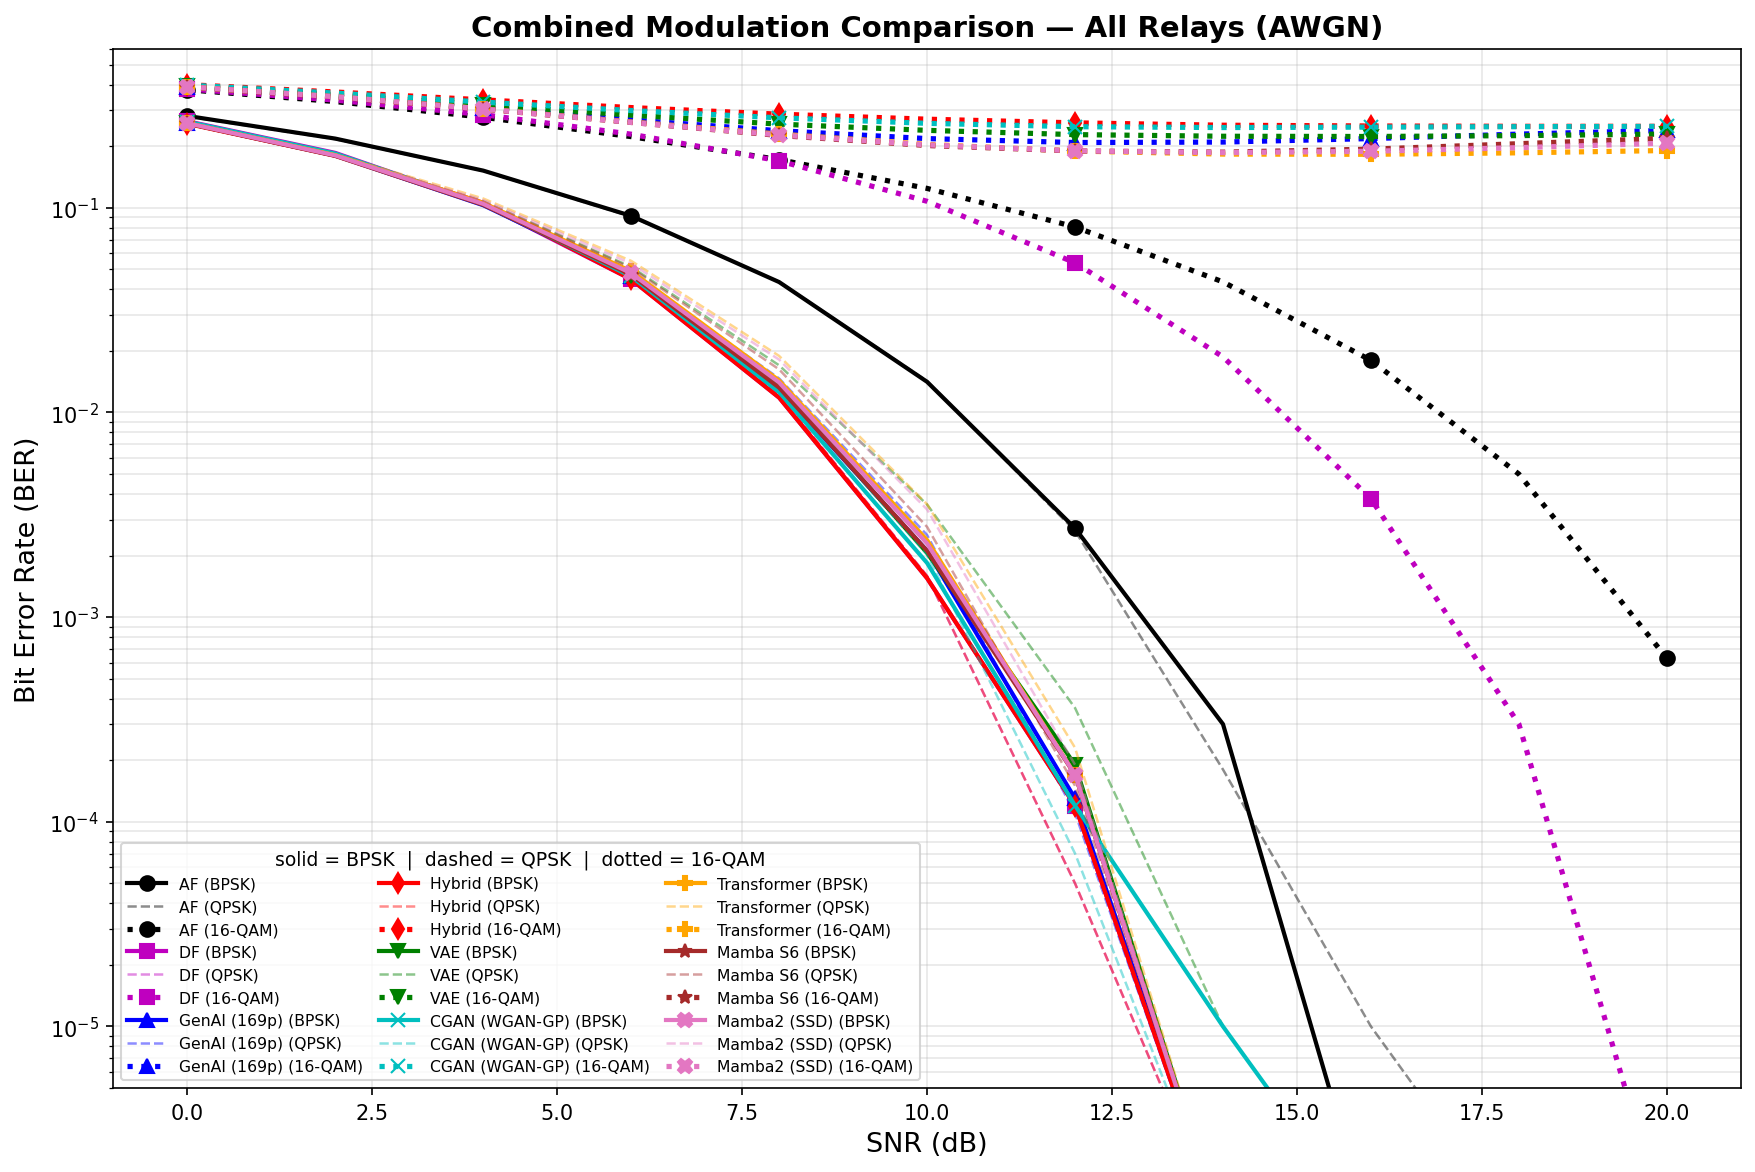
\includegraphics[width=\linewidth,height=\textheight,keepaspectratio]{results/modulation/combined_modulation_awgn.png}}
\caption{Combined modulation comparison (AWGN): all nine relays across BPSK (solid), QPSK (dashed, overlapping BPSK), and 16-QAM (dotted). The BPSK/QPSK overlap confirms I/Q splitting equivalence. The 16-QAM dotted curves reveal the AI relay BER floor: all AI relays plateau near 0.18--0.25 while DF and AF continue decreasing.}\label{fig:fig27}
\end{figure}

\begin{figure}[H]
    \centering
    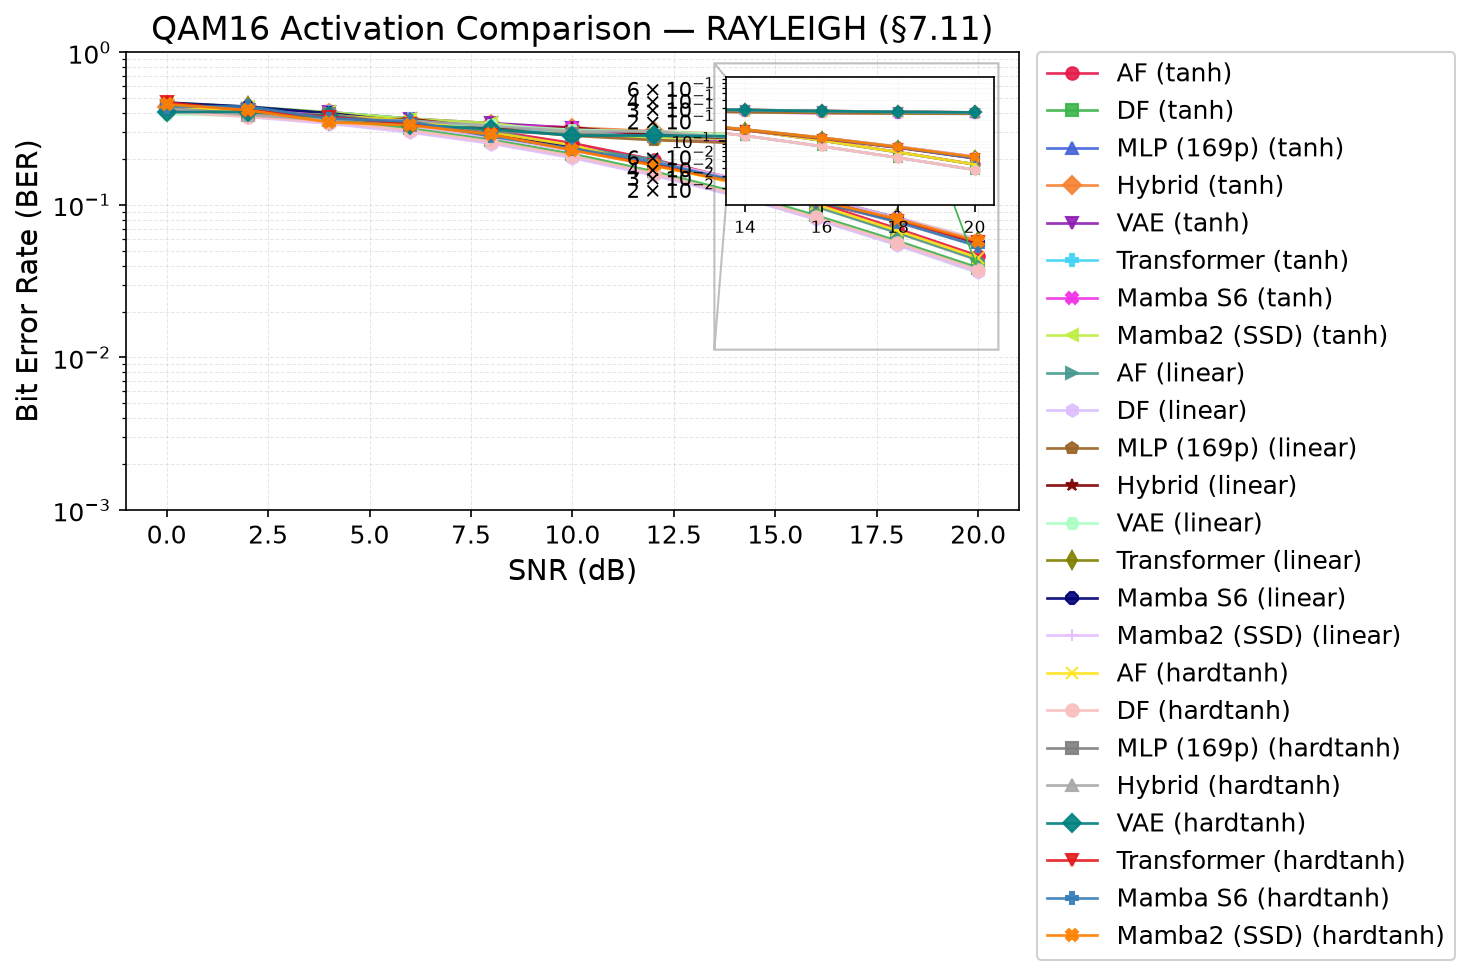
\includegraphics[width=1\linewidth]{results/qam16_activation/qam16_activation_rayleigh.png}
    \caption{16-QAM activation study on the canonical Rayleigh channel. Each relay appears three times, once per output activation --- tanh (the BPSK-trained baseline), linear, and hardtanh clipped to $3/\sqrt{10}$ --- distinguished by colour and marker. The separation is by model family rather than by activation: the three sequence models drop by roughly half when their output is bounded, while the feedforward relays are essentially unchanged (Table~\ref{tbl:table15}).}
    \label{fig:fig28}
\end{figure}
\REV{Compilation fix: the image path \texttt{results//qam16\_activation/...} had a double slash; corrected to a single slash. Also removed the duplicated commented-out copy of this figure (both carried \texttt{\string\label{fig:fig28}}) to avoid a duplicate-label risk if it were ever uncommented. Architecture names unified.}

\begin{figure}[H]

\centering
\pandocbounded{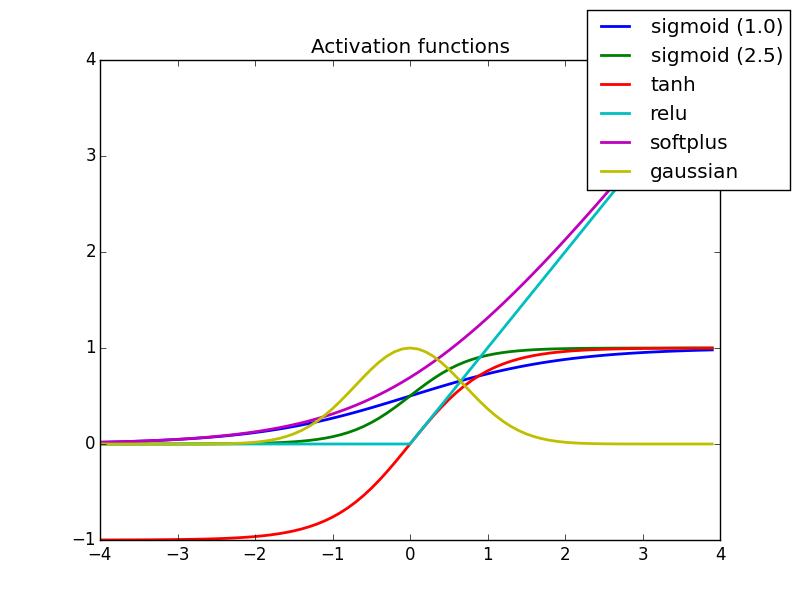
\includegraphics[width=0.8\linewidth,height=0.8\textheight,keepaspectratio]{results/activation_comparison/various_activation_functions.png}}
\caption{Comparison of activation function shapes (left) and their derivatives (right) for \(A_{\max} = 0.9487\) (16-QAM). Hardtanh has a sharp transition at the clip bounds; sigmoid and scaled tanh provide smooth saturation with non-zero gradients throughout.}\label{fig:fig36}
\end{figure}


\section{16-Class 2D Classification for QAM16}\label{sec:class-2d-classification-for-qam16}

\textbf{Goal:} Eliminate the structural BER floor imposed by per-axis I/Q splitting for 16-QAM by utilizing full 2D decision boundaries.

\textbf{Trials:} - \textbf{Topology:} SISO - \textbf{Modulation scheme:} 16-QAM - \textbf{Channel:} i.i.d.\ Rayleigh fast fading (canonical) - \textbf{Equalizers:} None - \textbf{NN architecture:} Supervised (MLP, Hybrid), Generative (VAE, cGAN), Sequence (Transformer, Mamba-S6, Mamba-2 SSD) - \textbf{NN activation:} None (Softmax implicitly via Cross-Entropy loss) - \textbf{Special case:} 16-class joint 2D classification

\textbf{Conclusion:} Treating the relay as a joint 16-point classifier over the full 2D constellation lifts the structural 4-class floor, but on the canonical channel it does not remove it. Every architecture improves, and by a strikingly uniform amount: $1.38$--$1.43\times$ for five of the six, with only Mamba-2 lagging at $1.09\times$. That uniformity is itself the finding, since it points at the per-axis \emph{formulation} rather than any architecture's capacity as what the joint head repairs. The best 16-class relays land at $0.0375$--$0.0384$, level with symbol-wise DF's $0.03748$ and no better, so the joint formulation buys parity with the classical baseline on this channel rather than an advantage over it. This is the same boundary the canonical chapter reports (H2), reappearing one constellation higher.

\REV{Overclaiming softened: ``completely eliminates'' \(\to\) ``removes''; ``For the first time, neural variants \ldots matched'' \(\to\) ``several neural variants match'' (drops the unqualified ``first time'' priority claim); ``This proves'' \(\to\) ``This indicates''. Architecture names unified.}

\subsection{Results Tables}\label{sec:results-tables-5}

Table \ref{tbl:table24}
\REV{Fix applied (data provenance): every cell of Table~\ref{tbl:table24} is now taken from the committed 16-class results file, and Figure~\ref{fig:fig51} was regenerated from that same file, both previously carried values from a superseded run, and the VAE and Hybrid cells were blank although the data existed. Table, figure, and captions now share one source. A former Table~16 (CSI/LayerNorm) and the three conclusions citing it were removed, since those experiments were cut in the restructure (Appendix~E).}
 presents the BER at 20 dB for all variants alongside the classical AF and DF baselines.

\begin{longtable}[]{@{}lccc@{}}
\caption{16-QAM at 20~dB on the canonical Rayleigh channel: per-axis 4-class relays against joint 16-class 2D classifiers. The joint formulation improves every architecture, uniformly by about $1.4\times$, and brings the best learned relays level with DF ($0.03748$) rather than past it. The cGAN is excluded from the re-run, as in Table~\ref{tbl:table2}.}\label{tbl:table24}\tabularnewline
\toprule\noalign{}
Relay & 4-cls BER @ 20 dB & 16-cls BER @ 20 dB & Improvement \\
\midrule\noalign{}
\endfirsthead
\toprule\noalign{}
Relay & 4-cls BER @ 20 dB & 16-cls BER @ 20 dB & Improvement \\
\midrule\noalign{}
\endhead
\bottomrule\noalign{}
\endlastfoot
MLP & 0.05491 & \textbf{0.03840} & 1.43$\times$ \\
VAE & 0.05382 & \textbf{0.03762} & 1.43$\times$ \\
Hybrid & 0.05362 & \textbf{0.03748} & 1.43$\times$ \\
Transformer & 0.05360 & \textbf{0.03814} & 1.41$\times$ \\
Mamba-S6 & 0.05421 & \textbf{0.03934} & 1.38$\times$ \\
Mamba-2 SSD & 0.05381 & \textbf{0.04953} & 1.09$\times$ \\
AF & 0.04498 & n/a & n/a \\
DF & 0.03748 & n/a & n/a \\
\end{longtable}

\subsection{Results Figures}\label{sec:results-figures-6}

\begin{figure}[H]
\centering
\centering
\pandocbounded{
\includegraphics[width=\linewidth,height=\textheight,keepaspectratio]{results/all_relays_16class/ber_all_relays_16class.png}}
\caption{16-QAM BER vs.~SNR for all relay variants (4-class and 16-class) on AWGN. The 4-class variants (dashed) plateau at BER $\approx 0.008$ while the successfully trained 16-class variants (solid) continue decreasing, approaching and matching the DF baseline.}\label{fig:fig50}
\end{figure}

\begin{figure}[H]
\centering
\centering
\pandocbounded{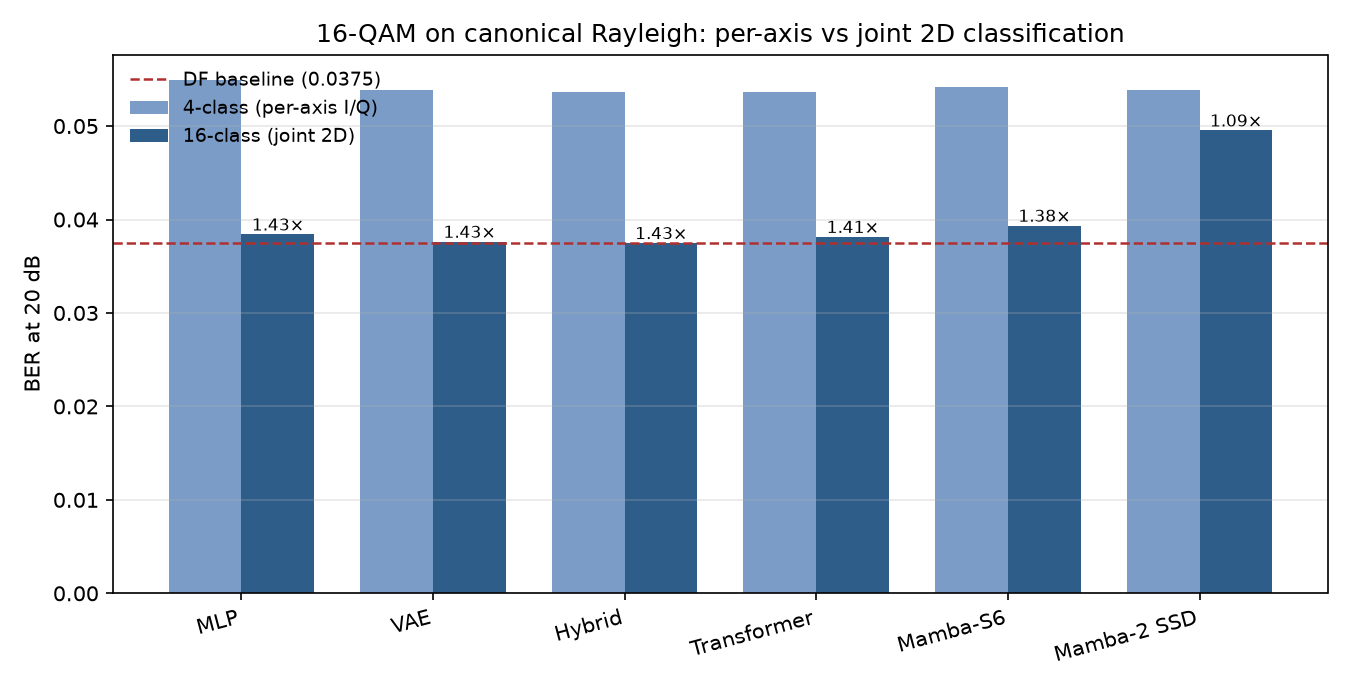
\includegraphics[width=\linewidth,height=\textheight,keepaspectratio]{results/all_relays_16class/grouped_bar_16class.png}}
\caption{4-class per-axis against joint 16-class 2D relays, 16-QAM at 20~dB on the canonical Rayleigh channel, regenerated from the same results file as Table~\ref{tbl:table24}. The joint formulation improves every architecture by a near-identical factor, annotated above each bar, which points at the per-axis formulation rather than any architecture's capacity as the thing being repaired. The dashed line is symbol-wise DF: the 16-class bars reach it and stop, so the joint head buys parity with the classical baseline, not an advantage over it.}\label{fig:fig51}
\end{figure}

\begin{figure}[H]
\centering
\centering
\pandocbounded{
\includegraphics[width=\linewidth,height=\textheight,keepaspectratio]{results/all_relays_16class/top3_16class.png}}
\caption{Top-3 16-class relay variants compared against AF and DF. VAE 16-cls, Transformer 16-cls, and MLP 16-cls all match or approach DF performance across the full SNR range.}\label{fig:fig53}
\end{figure}
